\newcommand{\dir}{../preface}

%========================= PREFACE ========================= 
\ifthenelse{\boolean{edthesis}}
 {
   \begin{prefacepart}
   \pagenumbering{roman} 
}
{
  \frontmatter
}

\thispagestyle{empty}

\begin{minipage}{\textwidth}
\end{minipage}
\begin{center}
\vspace{2cm}
{ \Huge A School of GeoScience PhD Thesis using {\LaTeX} 
  \par
  \vspace{0.5cm} 
{\Large Una Person \par}
}
\end{center}
\vfill
\begin{center}
\vspace{6cm}    
\centerline{
\epsfig{file=\dir/2Line2ColCMYK_CS3.eps,width=0.35\textwidth}}
\vspace{0.5cm}
Thesis submitted in fulfilment of\\
the requirements for the degree of\\ 
Doctor of Philosophy\\ 
to the\\
University of Edinburgh --- 2003
\end{center}

\newpage
\thispagestyle{empty}



\chapter{Declaration}
\vspace*{2\baselineskip}
I declare that this thesis has been composed 
solely by myself and that it has not been submitted, either in whole or
in part, in any previous application for a degree.
Except where otherwise acknowledged, the work presented is entirely my
own.
\vspace{6\baselineskip}\\
\begin{flushright}
\hspace*{\fill}
Una Person
\newline
September 2003
\end{flushright}


\cleardoublepage

\chapter{Abstract}
\markboth{\MakeUppercase{Abstract}}{\MakeUppercase{Abstract}}
The abstract...

\chapter{Acknowledgements}
\markboth{\MakeUppercase{Acknowledgements}}{\MakeUppercase{Acknowledgements}}

It's nice to acknowledge some people...


{\setlength{\parskip}{0ex plus 0.5ex minus 0.2ex}

\ifthenelse{\boolean{edthesis}}
 {
  \begin{singlespace}
 }{}

\tableofcontents
\listoftables
\listoffigures
% Glossary stuff
%\input{\dir/glossary.tex}
%\cleardoublepage
%\renewcommand{\nomname}{List of Symbols}
%\markboth{\MakeUppercase{\nomname}}{\MakeUppercase{\nomname}}
%\addcontentsline{toc}{chapter}{List of Symbols}
%\printglossary
\ifthenelse{\boolean{edthesis}}
 {
  \end{singlespace}
 }{}
}

\ifthenelse{\boolean{edthesis}}
 {
   \end{prefacepart}
   \pagenumbering{arabic} 
}
{
   \mainmatter
}
%========================= CHAPTERS ========================= 
\renewcommand{\dir}{../chapter1/chapter/}
\chapter{Template Chapter}
This is a template chapter. Lots of exciting stuff should go in here\footnote{testing a footnote}.


\begin{figure}[htbp]
  \centering
  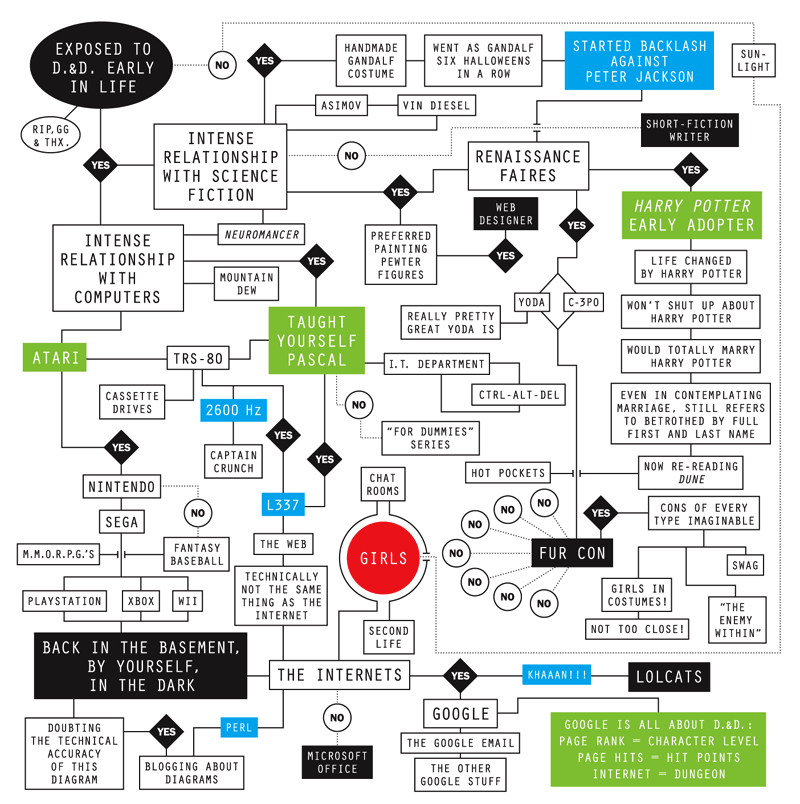
\includegraphics[width=0.7\textwidth]{\dir/figs/geek_flow_chart_nyt.png}
  \caption{an example figure from the \href{https://archive.nytimes.com/www.nytimes.com/imagepages/2008/03/09/opinion/09opart2.ready.html}{New York Times}...}
  \label{fig.example}
\end{figure}

Lorem ipsum dolor sit amet, consectetur adipiscing elit, sed do eiusmod tempor incididunt ut labore et dolore magna aliqua. Ut enim ad minim veniam, quis nostrud exercitation ullamco laboris nisi ut aliquip ex ea commodo consequat. Duis aute irure dolor in reprehenderit in voluptate velit esse cillum dolore eu fugiat nulla pariatur. Excepteur sint occaecat cupidatat non proident, sunt in culpa qui officia deserunt mollit anim id est laborum.

Lorem ipsum dolor sit amet, consectetur adipiscing elit, sed do eiusmod tempor incididunt ut labore et dolore magna aliqua. Ut enim ad minim veniam, quis nostrud exercitation ullamco laboris nisi ut aliquip ex ea commodo consequat. Duis aute irure dolor in reprehenderit in voluptate velit esse cillum dolore eu fugiat nulla pariatur. Excepteur sint occaecat cupidatat non proident, sunt in culpa qui officia deserunt mollit anim id est laborum.

Lorem ipsum dolor sit amet, consectetur adipiscing elit, sed do eiusmod tempor incididunt ut labore et dolore magna aliqua. Ut enim ad minim veniam, quis nostrud exercitation ullamco laboris nisi ut aliquip ex ea commodo consequat. Duis aute irure dolor in reprehenderit in voluptate velit esse cillum dolore eu fugiat nulla pariatur. Excepteur sint occaecat cupidatat non proident, sunt in culpa qui officia deserunt mollit anim id est laborum.

Lorem ipsum dolor sit amet, consectetur adipiscing elit, sed do eiusmod tempor incididunt ut labore et dolore magna aliqua. Ut enim ad minim veniam, quis nostrud exercitation ullamco laboris nisi ut aliquip ex ea commodo consequat. Duis aute irure dolor in reprehenderit in voluptate velit esse cillum dolore eu fugiat nulla pariatur. Excepteur sint occaecat cupidatat non proident, sunt in culpa qui officia deserunt mollit anim id est laborum.

\renewcommand{\dir}{../chapter2/chapter/}
\chapter{Template Chapter}
This is a template chapter. Lots of exciting stuff should go in here.


%========================= Appendix ========================= 
\renewcommand{\chaptermark}[1]{%
 \markboth{\MakeUppercase{%
 \appendixname} \ \thechapter.%
 \ #1}{}}
%\renewcommand{\dir}{../appendix/appendix}
%\input{\dir/appendix.tex}

%========================= BIBLIOGRAPHY ========================= 
\ifthenelse{\boolean{edthesis}}
 {
 \begin{singlespace}
}
{
  \backmatter
}
%\def\bibname{References}
%\tocotherhead{References}
%\addcontentsline{toc}{chapter}{References}
%\bibliography{ism}
\ifthenelse{\boolean{edthesis}}
 {
  \end{singlespace}
 }{}

